\documentclass[tikz]{standalone}
\usepackage{amsmath}
\usepackage{amsfonts}
\usepackage{amssymb}
\usepackage{tikz}
\usetikzlibrary{decorations.pathreplacing}
\usetikzlibrary{decorations.text}
\usetikzlibrary{arrows,shapes,backgrounds, shadows,fadings, calc, positioning, intersections}
\usepackage{pagecolor,lipsum}
\usepackage{color}
\definecolor{ColorA}{HTML}{286886}
\definecolor{ColorB}{HTML}{9EA0EE}
\definecolor{ColorC}{HTML}{740052}
\definecolor{ColorD}{HTML}{A76088}
\definecolor{A}{HTML}{F9F8EB}
\definecolor{B}{HTML}{FFE1B6}
\definecolor{C}{HTML}{7A9EB1}

\usepackage[nomessages]{fp}%

\def\Primary{{I,V,S,N,P,F,M}}

\usepackage{fontspec}
\setmainfont{Source Sans Pro}

\begin{document}

		%\pagecolor{A}
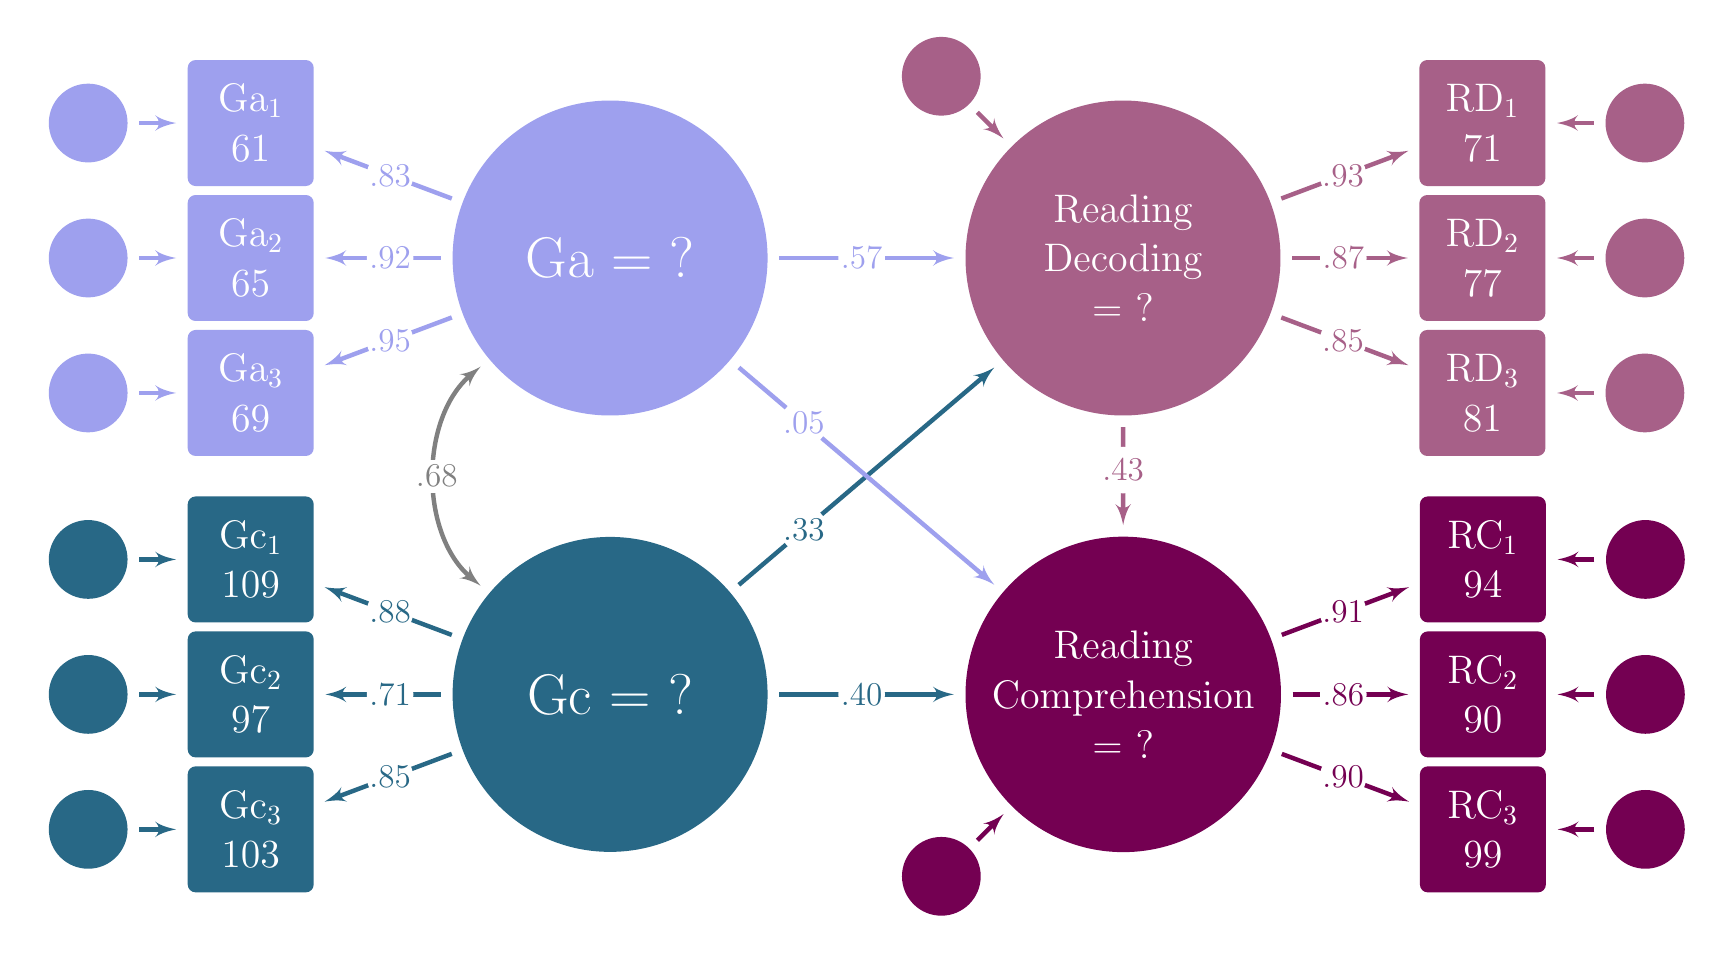
\begin{tikzpicture}[node distance=0.75cm,
latent/.style={
	circle,
	fill= black!30,
	minimum size=4cm,
	font=\huge,
	align=center,
	text = white},
latentlong/.style={
	circle,
	fill= black!30,
	minimum size=4cm,
	font=\Large,
	align=center,
	text = white},
error/.style={
	circle,
	text = white,
	fill = black!30,
	inner sep=1mm,
	minimum size=1cm,
	font=\normalsize},
ob/.style={
	rectangle,
	fill=black!30,
	minimum width=1.6cm,
	align=center,
	inner sep=0mm,
	minimum height=1.6cm,
	rounded corners = 1mm,
	font=\Large,
	text = white},
post/.style={
	->,
	draw,
	shorten >=4pt,
	shorten <=4pt,
	>=latex',
	ultra thick,
	color = black!50,
	text = black!50},
cov/.style={
	<->,
	shorten >=4pt,
	shorten <=4pt,
	>=latex',
	ultra thick,
	font=\Large,
	bend left=50,
	color = black!50,
	text = black!50,
	draw},
variance/.style={
	<->,
	>=latex',
	thick,
	bend left=245,
	looseness=4.5,
	shorten >=2pt,
	shorten <=2pt,
	font=\small,
	color = black!50,
	text = black,
	draw},
label/.style={
	fill=white,
	font=\large,
	circle,
%	fill = A,
	inner sep = 0mm}]


%Observed Vars



\node[ob, fill = ColorB]  (Ga1) at (1,0) {Ga\textsubscript{1}\\ 61};
\node[ob, fill = ColorB, below = 1mm of Ga1]  (Ga2) {Ga\textsubscript{2}\\ 65};
\node[ob, fill = ColorB, below = 1mm of Ga2]  (Ga3) {Ga\textsubscript{3}\\ 69};
\node[ob, fill = ColorA ,below = 5mm of Ga3]  (Gc1) {Gc\textsubscript{1}\\ 109};
\node[ob, fill = ColorA, below = 1mm of Gc1]  (Gc2) {Gc\textsubscript{2}\\ 97};
\node[ob, fill = ColorA, below = 1mm of Gc2]  (Gc3) {Gc\textsubscript{3}\\ 103};

\node[latent, right = 1.75cm of Ga2, fill = ColorB] (Ga) {Ga = ?};
\node[latent, right = 1.75cm of Gc2, fill = ColorA] (Gc) {Gc = ?};

\path[cov, bend left=50] (Gc) to node[label, rectangle, text = black!50, inner sep = 0.75mm]{.68} (Ga);



\path (Ga) to coordinate[pos = .45](center)   (Ga2);




\coordinate (up) at (center |- Ga1) ;
\coordinate (down) at (center |- Gc3);

\foreach \i/\load in {1/.83, 2/.92, 3/.95} {
	\path[post, ColorB] (Ga) to  (Ga\i);
	\node[label, text = ColorB] at (intersection of up--down and Ga--Ga\i) {\load};
	\node[error, fill = ColorB, left = of Ga\i] (eGa\i) {};
	\path[post, ColorB] (eGa\i) to (Ga\i);
}

\foreach \i/\load in {1/.88, 2/.71, 3/.85} {
	\path[post, ColorA] (Gc) to  (Gc\i);
	\node[label, text = ColorA] at (intersection of up--down and Gc--Gc\i) {\load};
	\node[error, fill = ColorA, left = of Gc\i] (eGc\i) {};
	\path[post, ColorA] (eGc\i) to (Gc\i);
}

\node[latentlong,right = 2.5cm of Ga, fill = ColorD] (RD) {Reading\\ Decoding\\ = ?};
\node[latentlong,right = 2.5cm of Gc, fill = ColorC] (RC) {Reading\\ Comprehension\\ = ?};

\path[post, ColorD] (RD) to node[label, pos = .450]{.43} (RC);
\path[post, ColorB] (Ga) to node[label, pos = .475]{.57} (RD);
\path[post, ColorA] (Gc) to node[label, pos = .270]{.33} (RD);
\path[post, ColorA] (Gc) to node[label, pos = .475]{.40} (RC);
\path[post, ColorB] (Ga) to node[label, pos = .270]{.05} (RC);


\node[ob, fill = ColorD, right = 1.75cm of RD]  (RD2) {RD\textsubscript{2}\\ 77};
\node[ob, fill = ColorD, above = 1mm of RD2]  (RD1) {RD\textsubscript{1}\\ 71};
\node[ob, fill = ColorD, below = 1mm of RD2]  (RD3) {RD\textsubscript{3}\\ 81};
\node[ob, fill = ColorC, right = 1.75cm of RC]  (RC2) {RC\textsubscript{2}\\ 90};
\node[ob, fill = ColorC, above = 1mm of RC2]  (RC1) {RC\textsubscript{1}\\ 94};
\node[ob, fill = ColorC, below = 1mm of RC2]  (RC3) {RC\textsubscript{3}\\ 99};

\path (RD) to coordinate[pos = .45](center)   (RD2);
\coordinate (up) at (center |- RD1) ;
\coordinate (down) at (center |- RC3);

\foreach \i/\load in {1/.93, 2/.87, 3/.85} {
	\path[post, ColorD] (RD) to  (RD\i);
	\node[label, text = ColorD] at (intersection of up--down and RD--RD\i) {\load};
	\node[error, fill = ColorD, right = of RD\i] (eRD\i) {};
	\path[post, ColorD] (eRD\i) to (RD\i);
}

\foreach \i/\load in {1/.91, 2/.86, 3/.90} {
	\path[post, ColorC] (RC) to  (RC\i);
	\node[label, text = ColorC] at (intersection of up--down and RC--RC\i) {\load};
	\node[error, fill = ColorC, right = of RC\i] (eRC\i) {};
	\path[post, ColorC] (eRC\i) to (RC\i);
}

\node[error, fill = ColorD, above left = of RD] (dRD) {};
\path[post, ColorD] (dRD) to (RD);

\node[error, fill = ColorC, below left =of RC] (dRC) {};
\path[post, ColorC] (dRC) to (RC);

\node[xshift = -1ex] at (current bounding box.south west){};
\node[xshift = 1ex] at (current bounding box.north east){};
	\end{tikzpicture}
\end{document}
